\documentclass[11pt]{beamer}
\usepackage{lmodern}
\usepackage{graphicx}
\usepackage{hyperref}
\usetheme{Singapore}
\author{Gerd Graßhoff}
\title{Algorithmische Geschichte und Philosophie der Wissenschaften, Vorl 7}
\date{27. Juli 2019}

\begin{document}
	\begin{frame}[plain]
		\maketitle
	\end{frame}
	

\section{Artikel, Abstract 14500}

	\begin{frame}
	\frametitle{Begriffserkennung}


\begin{figure}
	\centering
	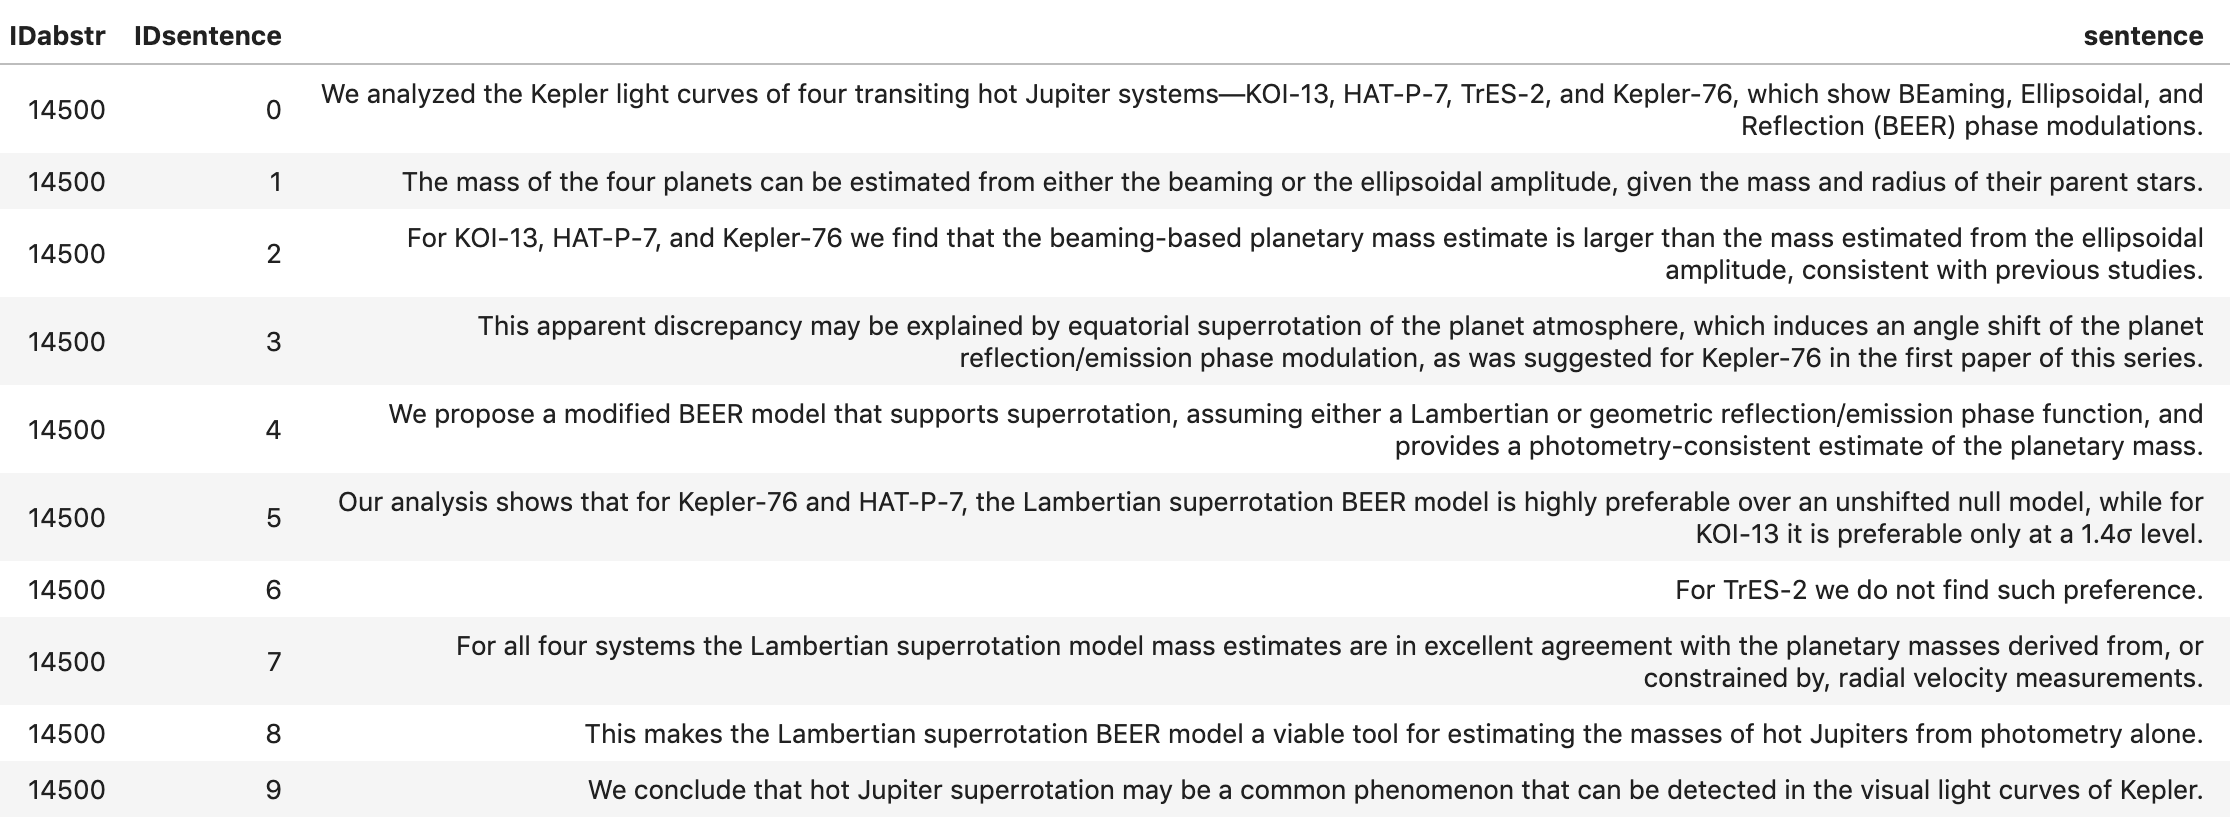
\includegraphics[width=1\linewidth]{screenshot001}
	\caption{Abstract 14500}
	\label{fig:screenshot001}
\end{figure}

\end{frame}

\begin{frame}
\frametitle{Attribute}

\begin{description}
	\item[EmpiricalData] Kepler light curves
	\item[ModelDescription] transiting hot Jupiter systems
	\item[ObjectName] KOI-13, HAT-P-7, TrES-2, and Kepler-76
	\item[EmpiricalData] BEaming, Ellipsoidal, and Reflection (BEER) phase modulations
	\item[ModelAttribute] The mass of the planet
	\item[EmpiricalData/ModelAttribute] beaming or the ellipsoidal amplitude
	\item[ModelAttribute] mass and radius of their parent stars.
	\item[ModelAttribute]equatorial superrotation of the planet atmosphere
	\item[ModelAttribute] angle shift of the planet reflection/emission phase modulation
	\item[ModelDescription]Lambertian superrotation BEER model	
	\item[EmpiricalData]radial velocity measurements
	\item[ModelDescription] hot Jupiter superrotation
\end{description}

\end{frame}

\begin{frame}
	\frametitle{Kategorien}
	
	\begin{description}
		\item[ObjectName] KOI-13, HAT-P-7, TrES-2, and Kepler-76
		\item[EmpiricalData] Kepler light curves
		\item[EmpiricalData] BEaming, Ellipsoidal, and Reflection (BEER) phase modulations
		\item[EmpiricalData] beaming or the ellipsoidal amplitude
		\item[EmpiricalData]radial velocity measurements
		\item[ModelDescription] transiting hot Jupiter systems
		\item[ModelDescription]Lambertian superrotation BEER model	
		\item[ModelDescription] hot Jupiter superrotation
		\item[ModelAttribute] The mass of the planet
		\item[ModelAttribute] mass and radius of their parent stars.
		\item[ModelAttribute]equatorial superrotation of the planet atmosphere
		\item[ModelAttribute] angle shift of the planet reflection/emission phase modulation
	\end{description}
	
\end{frame}

\begin{frame}
	\frametitle{Kategorien}

\href{https://spacy-vis.apps.allenai.org/spacy-parser}{Parser}

\end{frame}




\end{document}